\documentclass[utf8]{article}

\usepackage[utf8]{inputenc}

\usepackage[parfill]{parskip}

\usepackage{floatrow}
\usepackage{amsmath}
\usepackage{amssymb}
\usepackage{amsfonts}
\usepackage{graphicx}
\usepackage{float}
\usepackage{listingsutf8}
\usepackage{multirow}

\usepackage{fullpage}

% -----------------------------------------------------


\title{INFO-F201 SmallDB : rapport}
\author{HENNEBICQ Jérémy\and MARKOWITCH Romain \and MARNETTE Pol}
\date{16 décembre 2022}

\renewcommand{\contentsname}{Table des matières}
\begin{document}
\maketitle
\tableofcontents

\newpage

% -----------------------------------------------------

\section{Introduction}

Ce projet est la prolongation de la première partie \texttt{tinydb} en prenant une nouvelle approche. Le but est le même : la réalisation d'une base de données en C++. Ici le serveur est différencié du client et communiquent ensemble via des sockets. Aussi, les requêtes des différents clients seront maintenant gérées par des threads individuels. Cette nouvelle approche soulève des questions concernant l'implémentation. Il faudra faire attention au niveau de l'accès concurrent à la base de données, trouver un moyen de passer les réponses au client, etc.

Dans ce rapport nous allons décrire notre implémentation, revenir sur certains points qui nous ont posé problème et comparer cette nouvelle implémentation à la précédente.

\section{Implémentation serveur client}

\subsection{Implémentation des mutex}


Pour éviter les accès concurrents à la base de données, nous avons du implémenter des mutex. Nous avons utilisé le pseudo-code fournit dans l'énoncé pour créer 4 fonctions qui sont appelées avant et après les lectures et les écritures. L'implémentation de celles-ci se trouve dans le fichier \texttt{guard.cpp}. Voici l'explication de leurs fonctionnements :

\begin{enumerate}
	\item Nous créons une mutex \texttt{new\_access} qui sera utilisée pour bloquer le processus de registration du lecteur ou de l'écrivain. Elle sera bloquée au début de chaque fonction \texttt{\_before} et unlock à la fin,
	\item Nous créons une mutex \texttt{write\_access} qui permet de restreindre l'accès à un unique écrivain à la fois. La fonction \texttt{write\_guard\_before} la verrouillera et la fonction \texttt{write\_guard\_after} la déverrouillera,
	\item Nous créons une mutex \texttt{reader\_registration} qui restreindra l'accès à la variable \texttt{readers\_count} pour éviter que deux threads la modifient en même temps,
	\item Ensuite, dans la fonction \texttt{read\_guard\_before} on regarde s'il n'y a pas encore de lecteur, si c'est le cas, nous bloquerons l'écriture et incrémenterons le nombre de lecteur,
	\item Finalement dans la fonction \texttt{read\_guard\_after} on décrémentera le nombre de lecteur et si celui-ci est maintenant à 0, nous déverrouillerons l'accès à l'écriture.
\end{enumerate}

Cette approche empêche les écrivains de bloquer les lecteurs en permettant aux lecteurs de continuer à accéder à la base de données tant qu'il y a des lecteurs en cours d'exécution. Lorsqu'un lecteur termine, il décrémente le compteur de lecteurs et, s'il est égal à zéro, débloque l'accès en écriture pour les écrivains. De cette manière, cette implémentation de mutex permet d'éviter les problèmes de famine en gérant de manière efficace l'accès en lecture/écriture à la base de données.

\subsection{Difficultés rencontrées}

\subsubsection{Communication des résultats au client}


Pour communiquer les résultats d'une requête envoyée par le client au serveur nous avons d'abord essayé de transmettre au client un structure \texttt{query\_result\_t}. Cette structure contient un \texttt{std::vector} des étudiants sélectionnés, la requête, le type de requête (\texttt{SELECT}, etc), l'état de la requête et éventuellement un message d'erreur. Nous avons donc essayé d'envoyer cette structure au client pour qu'il puisse lire les résultats de sa requête. Voici le bout de code que nous avons essayé :

\begin{lstlisting}
write(socket, &query_result, sizeof(query_result_t));
\end{lstlisting}
	
	Nous n'avons pas réussi à faire fonctionner la communication avec cette approche. Nous en avons déduit que communiquer un \texttt{std::vector} via les sockets n'était pas trivial. Nous avons aussi essayé avec une liste dans le style de C (avec des pointeurs) mais le soucis restait.
	
	Dans uns second temps, nous avons opté pour une autre solution : envoyer ligne par ligne les résultats à imprimer chez le client. Nous avons défini un marqueur d'arrête (\texttt{**} en l'occurence) qui indiquera au client la fin des réponses à afficher dans le terminal. Cette solution fonctionne mais nous laisse perplexe au niveau de la charge réseaux et du nombre d'appels système. Une autre implémentation nécessitant moins de \texttt{read} et \texttt{write} pourrait être plus optimal. Voici une illustration de notre implémentation :

\begin{lstlisting}
// Server
for (auto student: query_result.students) {
	student_to_str(buffer_response, &student, 1024);
	write(socket, buffer_response, 1024);
}
snprintf(buffer_response, 1024, "%s", RESULT_EN_MARKER.c_str());
write(socket, buffer_response, 1024);

// Client 
while ((bytes_read = read(sock, response_buffer, 1024)) > 0
	&& strcmp(response_buffer, RESULT_EN_MARKER.c_str()) != 0) {
	std::cout << response_buffer << std::endl;
}
\end{lstlisting}

Afin d'essayer de résoudre un problème d'affichage lors de l'envoi en réseau (plus d'information à ce sujet dans la section dédiée), nous avons revu cette approche pour ne pas afficher dans le terminal chaque \texttt{read} mais de l'ajouter à un string \texttt{response} et une fois le marqueur détecté à la fin de ce string, afficher \texttt{response} dans le terminal.

\subsubsection{Nombre d'étudiants supprimés}

Quand un client exécute la requête \texttt{delete filter=value}, le serveur supprime les éléments et renvoie au client \texttt{n student(s) deleted}. Le code fournit pour ce projet contenait déjà la logique de la fonction delete mais pas un moyen de récupérer facilement le nombre d'étudiants supprimés. Cette fonction utilise \texttt{remove\_if} qui retourne un itérateur sur le vecteur. Pour compter les éléments nous avons itéré sur les éléments supprimés pour les compter. Voici un bout de code de l'implémentation :

\begin{lstlisting}
auto new_end = remove_if(db->data.begin(), db->data.end(), predicate);

for (auto s = new_end; s != db->data.end(); ++s) {
	query_result.students.push_back(*s);
}
\end{lstlisting}

\subsubsection{Communication sur différentes machines}

Nous avons rencontré un problème lors de nos tests sur différentes machines : quand un des deux ordinateurs est un serveur (\texttt{smalldb}) et que l'autre est le client (\texttt{sdbsh}).

Dans un premier temps, nous avons testé sur un partage de connexion via un iPhone mais certains des résultats retournés par le serveur étaient étranges.

\begin{figure}[ht]
	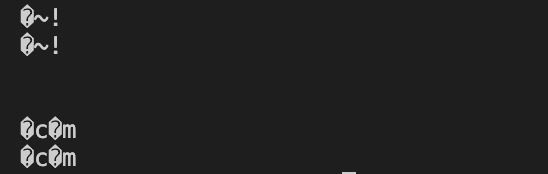
\includegraphics[scale=0.6]{assets/char-iphone.png}
	\caption{Exemple des résultats retournés par le client lors d'une connexion à un serveur sur un réseau local via le partage de connexion.}
	\label{fig:char_iphone}
\end{figure}

Nous nous sommes dit que cela pouvait être une limitation du routeur interne à l'iPhone lors du partage de connexion. Pour tester d'une autre manière nous avons donc lancé \texttt{smalldb} sur un serveur distant loué chez Hetzner pour l'occasion. Nous arrivons à nous connecter correctement sur ce serveur distant, nous arrivons aussi à sélectionner des étudiants et ceux-ci s'affichent bien. Cependant, à la fin du select des caractères étranges s'affichent, principalement quand le select retourne plus d'un étudiant.

\begin{lstlisting}
> ./sdbsh 142.132.176.27
> select fname=Pol
000000001: Pol Marnette in section INFO, born on the 12/07/2001
1 student(s) selected
> select section=INFO
000000001: Pol Marnette in section INFO, born on the 12/07/2001
000000002: Romain Markowitch in section INFO, born on the 05/05/2003
000000003: Jeremy Hennebicq in section INFO, born on the 06/12/2003
3 student(s) selected
V
V
\end{lstlisting}

Les deux \texttt{V} qui s'affichent ne sont pas attendus. Aussi, le client n'arrive pas à détecter que le serveur a fini de lui retourner les résultats et il n'est alors pas possible de renvoyer une nouvelle requête via le client.

Nous avons tenté de résoudre ce problème en modifiant la manière dont le client reçoit et affiche les résultats (comme détaillés dans le point "Communication des résultats au client") mais ceci n'a pas résolu le problème. Cette solution nous a seulement permis d'éviter l'affichage des caractères spéciaux mais le client restera bloqué et aucune autre requête ne pourra être envoyée.


\section{Bash}

\subsection{Fonctionnement}

Nous avons décidé de faire un code le plus simple possible. Pour ce faire, comme toutes les fonctions demandées utilisent le PID du processus \texttt{smalldb}, nous avons créé une variable globale PID qui grep \texttt{smalldb} (récupère le PID du processus de \texttt{smalldb}). Ensuite il nous restait plus qu'à envoyer un signal \texttt{SIGINT} pour la fonction stop (arrêter le serveur) :

\begin{lstlisting}
stop(){
kill -SIGINT $pid
}
\end{lstlisting}

Un signal \texttt{SIGUSR1} pour la fonction sync (sauvegarde la base de données sur le disque) :

\begin{lstlisting}
sync(){
kill -SIGUSR1 $pid
}
\end{lstlisting}

Et enfin récupérer l'adresse IP des clients grâce à la fonction list : 

\begin{lstlisting}
list(){
lsof -i -P -n | grep "$pid" | awk '{print $9}' | cut -d- -f2 | \
sed 's/>//g' | cut -d: -f1 | sed '1d'
}
\end{lstlisting}

Les paramètres utilisés dans la fonction \texttt{lsof} sont expliqués dans le fichier \texttt{smalldbctl} et les problèmes rencontrés sont quant à eux expliqués dans la sous-section ci-dessous.

\subsection{Difficultés rencontrées}

Lors de la création de la fonction \texttt{list}, un problème est survenu avec l'affichage de l'adresse IP. La commande \textt{ss} était introuvable sur Mac et \texttt{netstat} ne fonctionnait pas avec les options nécessaires pour récupérer l'IP voulu.

Nous avons donc dû trouver une autre commande nous permettant de récupérer l'IP du client.

Après de longues heures de recherche nous avons trouvé la commande \texttt{lsof}. Mais un nouveau problème apparu, il fallait trier les informations que la commande \texttt{lsof} affichait. Nous avons trouver grâce à des forums (dont Stack Overflow) comment récupérer ce que \texttt{lsof} affichait, comment en extraire la partie voulue, la séparer à partir d'un certain symbole ("-" dans notre cas) et aussi comment sélectionner la bonne partie après un cut. Après ça il ne nous restait plus qu'à retirer l'astérisque qui s'affichait avant les IP à l'aide la commande \texttt{sed/'1d'} qui retire la première ligne de notre echo (en bash).

\section{Tests additionnels}

Afin de tester notre implémentation, nous avons dans un premier temps créé une "Github Action" pour compiler afin tester notre code à chaque nouveaux commit. Celui-ci se contentait de lancer \texttt{make} afin de compiler le code et lançait ensuite le script bash fournit qui contient les différents tests. Dans un second temps, comme mentionné dans la partie sur les difficultés rencontrés, nous avons déployé la partie \texttt{smalldb} (le serveur) sur une machine virtuelle distante pour tester notre code dans des conditions plus concrètes.

Concernant le fichier \texttt{/tests/run\_tests.sh}, nous avons ajouté un \texttt{sleep 0.5} entre le lancement du serveur et du client car sinon, le client se lançait avant que le serveur n'ait eu le temps de commencer à accepter de nouvelles connections. Ceci provoquait alors une erreur lors des tests en fonction de la machine sur laquelle ceux-ci étaient lancés.

\section{Comparaison avec la première partie}

\subsection{Pipe et sockets}

Un des changements majeur qu'apporte la seconde partie du projet est la communication via sockets entre le client et le serveur. Dans la première partie, nous utilisions les pipes, non pas pour communiquer entre le client et le serveur mais pour communiquer entre les processus gérants les requêtes et le processus principale qui communique avec l'utilisateur.

Cette nouvelle approche se rapproche plus de ce que l'on pourrait retrouver en réalité avec un serveur distant du client.


\subsection{Processus et threads}

Dans cette nouvelle partie, nous exécutons les requêtes des clients de manière parallèle sur des threads différents. Dans la première partie, nous avions séparé l'exécution de chaque type de requête dans des processus différents.

Les threads sont d'une plus grande flexibilité pour cette implémentation. Par exemple, partager la base de données est maintenant plus simple mais si elle requiert l'utilisation de mutex.

Le fait de paralléliser les requêtes des clients au lieu de paralléliser les types de requêtes comme dans la partie 1 rend l'implémentation plus scalable et ainsi nous semble plus se rapprocher d'un cas de la vie réelle.


\subsection{Bash}

La partie Bash du projet 2  a été plus simple - réaliser que celle de la partie 1.
Pour la première partie, le nombre d'arguments rentrés pouvait modifier le comportement des fonctions alors que dans la seconde partie, le seul argument à entrer est le nom de la fonction appelée.

Dans la seconde partie, il suffit de récupérer le PID de \texttt{smalldb} et de lui envoyer un signal. Tandis que pour la partie 1 nous devions trouver le bon PID parmi les différents processus en cours, pour pouvoir lui envoyer le signal voulu. Cette recherche du bon PID demandait un traitement plus conséquent avant l'envoie du signal, par rapport au simple envoie du signal de la partie 2. 

\end{document}
